\section{Methodology}
\subsection{Outline}
This section will look into analysis of the six DOF Stewart platform, considerations for the force sensor and the velocity measurement within the wind tunnel. It will finally look into the design of a human machine interface that will be used to control the Stewart platform, obtain measurements and display results.

\subsection{Mechanical Design}
Since a Stewart platform has already been designed and fabricated, this section will look at: design considerations and analysis and evaluation of the Stewart platform to verify whether it will be feasible to work with.
\subsubsection{Design Considerations for the Stewart Platform}
\begin{enumerate}
\item When the controllable axes are active, the platform must be controlled in six degrees of motion.
\item When the controllable members are stationary, the
platform must have a corresponding fixed position.
\item The design parameters for consideration are: mobile platform radius, height of the platform and angle between adjacent joints of mobile platform and base plate.
\item The mechanism should be lightweight.
\item Velocity and position control of the mechanism should be easy to achieve.
\end{enumerate}
%\subsection{Kinematic Analysis - Rotational matrix}
%Euler angles are utilized to obtain rotational matrix for the moving platform of the Stewart platform mechanism. The rotational matrix is represented as follows \cite{csumnu2017simulation}:
%\begin{ceqn}
% R_{P}^B = R_{Z}(\gamma)*R_{Y}(\beta)*R_{X}(\alpha)
%\end{ceqn}
%Where $\gamma, \beta, \alpha$ - angles of rotation about the z-, y- and x-axis respectively.

%In matrix form:
%\[ R_{P}^B =
% \begin{bmatrix}
% c\beta c\gamma & s\alpha s\beta c\gamma - c\alpha s\gamma & c\alpha s\beta c\gamma + s\alpha s\gamma\\
% c\beta s\gamma & s\alpha s\beta s\gamma + c\alpha c\gamma & c\alpha s\beta s\gamma - s\alpha c\gamma\\
% -s\beta & s\alpha c\beta & c\alpha c\beta  
% \end{bmatrix}
%\]
%Generalized coordinate position and velocity vector of the moving platform is represented below \cite{csumnu2017simulation}:
%\[
%q=
%\begin{bmatrix}
%tx & ty & tz & \alpha & \beta & \gamma
%\end{bmatrix}^\top
%\]
%\[
%\dot{q}=
%\begin{bmatrix}
%\dot{tx} & \dot{ty} & \dot{tz} & \dot{\alpha} & \dot{\beta} & \dot{\gamma}
%\end{bmatrix}^\top
%\]
%Transformation of angular velocity of moving platform to the base frame can be done using Euler angles \cite{csumnu2017simulation}:
%\[
%\omega =
%\begin{bmatrix}
%1 & 0 & s\beta \\
%0 & c\alpha & -s\alpha c\beta \\
%0 & s\alpha & c\alpha c\beta 
%\end{bmatrix}
%\begin{bmatrix}
%\dot{\alpha} \\
%\dot{\beta}\\
%\dot{\gamma}
%\end{bmatrix}
%\]
%Acceleration of the moving platform is obtained by differentiating the velocity of the moving platform with respect to time:
%\[
%\dot{\omega} =
%\begin{bmatrix}
%1 & 0 & s\beta \\
%0 & c\alpha & -s\alpha c\beta \\
%0 & s\alpha & c\alpha c\alpha c\beta 
%\end{bmatrix}
%\begin{bmatrix}
%\ddot{\alpha} \\
%\ddot{\beta}\\
%\ddot{\gamma}
%\end{bmatrix}
%+
%\begin{bmatrix}
%0 & 0 & \dot{\beta}c\beta \\
%0 & \dot{\alpha} s\alpha & -\dot{\alpha} c\alpha c\beta + s\alpha \dot{\beta} s\beta \\
%0 & \dot{\alpha}c\alpha & -\dot{\alpha}s\alpha c\beta - c\alpha \dot{\beta}s\beta
%\end{bmatrix}
%\begin{bmatrix}
%\dot{\alpha} \\
%\dot{\beta}\\
%\dot{\gamma}
%\end{bmatrix}
%\]
%\subsection{Inverse Kinematic Analysis}
%Inverse kinematic analysis is used to determine the length of the legs according to planned trajectories of the moving platform position. In order to consider the length of the leg of a Stewart platform, closed-loop of one leg is used as shown in figure 3.1. Using this closed-form representation, the leg
%vector with respect to base platform can be obtained as follows \cite{csumnu2017simulation}:
%\begin{ceqn}
%\label{eqn}
%L_{i} = q_{i}^{B} - b_{i}
%\end{ceqn}
%The position vector of ith upper junction point with respect to the base frame is given by the following;
%\begin{ceqn}
%\label{eqn}
%q_{i}^{B} = t + R_{p}^{B} * q_{i}^{p}
%\end{ceqn}
%\begin{center}
%	\begin{figure}[!h]
%	\centering
%	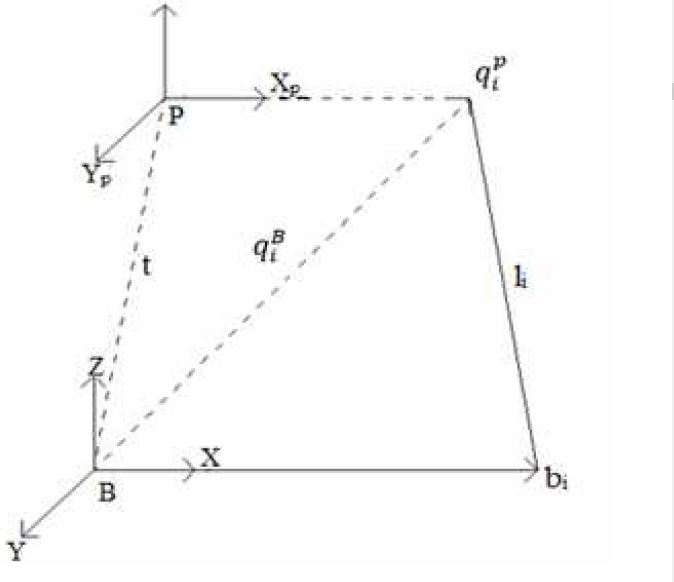
\includegraphics[width=0.6\linewidth]{Figures/Fig12}
%	\caption[Closed-loop representation]{Closed-loop representation of one leg of the Stewart Platform \cite{csumnu2017simulation}}
%	\end{figure}
%\end{center}
%Then the length of the ith leg can be acquired as follows:
%\newpage
%\begin{multline}
%\label{eqn}
%l_{i}^2 = (a_{x} * r_{p} * c_{i} + b_{x}*r_{p}*s_{i}
%+ t_{x}-r_{b}*c_{i})^2 + \\(a_{y}*r_{p}*c_{i} + b_{y}*r_{p}*s_{i} + t_{y}-r_{b}*s_{i})^2+ (a_{z}*r_{p}*c_{i}+b_{z}*r_{p}*s_{i}+t_{z})^2
%\end{multline}
%\subsection{Inverse Velocity Analysis}
%Inverse Jacobian matrix can be used to perform inverse velocity analysis of the Stewart
%platform. Inverse Jacobian matrix describes relation between velocity of the moving platform and the leg velocity.

%Inverse Jacobian matrix for a 6-DOF Stewart Platform
%\cite{csumnu2017simulation}:
%\[ J^-1 =
%\begin{bmatrix}
%u_{1}^{T} & (R_{P}^{B}q_{1}^{B} * u_{1})^T\\
%u_{2}^{T} & (R_{P}^{B}q_{2}^{B} * u_{2})^T\\
%u_{3}^{T} & (R_{P}^{B}q_{3}^{B} * u_{3})^T\\
%u_{4}^{T} & (R_{P}^{B}q_{4}^{B} * u_{4})^T\\
%u_{5}^{T} & (R_{P}^{B}q_{5}^{B} * u_{5})^T\\
%u_{6}^{T} & (R_{P}^{B}q_{6}^{B} * u_{6})^T
%\end{bmatrix}
%\]
\subsubsection{Base and Moving Platform}
 The Stewart platform should be stable. Thus the base should have a larger diameter than that of the moving platform. The Center of Gravity (COG) shouldn't fall outside the base during any of the platform movements.
 \subsubsection{Stewart Platform Configurations}
Stewart platforms can take three primary configurations i.e. 3-3 type, 3-6 type or 6-6 type.
\begin{center}
	\begin{figure}[H]
	\centering
	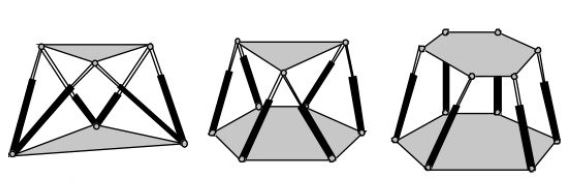
\includegraphics{Figures/stewart}
	\caption[Configurations]{Type 3-3, 3-6 and 6-6 respectively
	\cite{fernandes_design_nodate}}
	\end{figure}
\end{center}
The base and the platform (for the 3-3 type), and the platform (for the 3-6 type) are triangular in shape. The triangular shape has a good load carrying capability only in theory and for certain dimensions. These configurations are, however,not possible in practice since double spherical joints will be needed where two bars have to be joined at the same vertex
\cite{fernandes_design_nodate}.

The platform is a a 6-6 type. The base and platform are hexagon in shape.

\subsubsection{Quality Index $(\lambda)$ of Stewart Platform Design}
Quality index $(\lambda)$ varies from 0 to 1.\\
Where,\\
0 - design with singularities and\\
1 - Optimal design in which the determinant of the correspondent Jacobian matrix is maximum.

\textbf{Singularities} - uncontrollable states.

Derivation of the formula to compute the quality index has been done and is presented in the literature review.

Taking the Stewart Platform base diameter of 300mm, platform diameter of 200mm and height of 190mm i.e.: 

a = 200mm, b = 300mm, h = 190mm , $\alpha = 0.25$, $ \beta = 0.1667$,
\begin{ceqn}
\begin{align}
	|J| =
	\frac{81 \sqrt{3} a^3 b^3 h^3 (3 \alpha \beta - 2 \alpha - 2 \beta +1)^3}{4(a^2(3 \alpha^2 - 3 \alpha + 1)+ ab(\alpha \beta - 1 )+ b^2(3 \beta^2 - 3 \beta + 1)+ 3h^2)^3} = 2.437 \times 10^{-3}
	\label{eq:myeqn}
\end{align}
\end{ceqn}
And $ |J|_{m}$ where,
\begin{ceqn}
\begin{align}
	h = \sqrt{\frac{1}{3}(a^2 (3 \alpha^2 - 3 \alpha + 1)+ ab (3\alpha\beta - 1)+b^2(3 \beta^2 - 3 \beta + 1))} = 0.0764
	\label{eq:myeqn}
\end{align}
\end{ceqn}
\begin{equation*}
|J|_{m} =
\frac{81 \sqrt{3} a^3 b^3 h^3 (3 \alpha \beta - 2 \alpha - 2 \beta +1)^3}{4(a^2(3 \alpha^2 - 3 \alpha + 1)+ ab(\alpha \beta - 1 )+ b^2(3 \beta^2 - 3 \beta + 1)+ 3h^2)^3} = 2.834 \times 10^{-3}
\label{eq:myeqn}
\end{equation*}
Quality index for this Stewart Platform design is therefore, 

$$\lambda = \frac{|J|}{|J|_{m}} = 0.86$$
%\label{eq:myeqn}
%A quality index of 0.86 presents a design of high quality and mechanical feasibility.
\subsubsection{Sheet Metal Thickness and Material}
Metal used to manufacture the base should be of significant thickness to provide more support to the whole structure.

Metal used to manufacture the moving platform should be lightweight and of enough thickness to enable it to withstand significant loads.

Some sheet metal materials are considered and compared in table \ref{table1}.

\begin{center}
\begin{table}[!h]
	\caption[Sheet Metal Properties]{Material Properties}
	\label{table1}
\centering
\begin{tabular}{|l|l|l|}
\hline
\textbf{Metal} & \textbf{Density$(gcm^{-3})$} & \textbf{Yield Strength(MPa)}\\
\hline
Aluminium (6061-T6)& 2.7 & 270\\
\hline
Mild Steel & 7.85 & 250\\
\hline
Stainless Steel & 7.5 - 8.0 & 215\\
\hline
\end{tabular}
\end{table}
\end{center}
Aluminium 6061 is preferable for the moving platform since it is lightweight and can withstand significant loads without yielding. It also has good machinability (50 per cent). A sheet metal of 1.5mm thickness is used for the platform.
\begin{center}
	\begin{figure}[H]
	\centering
	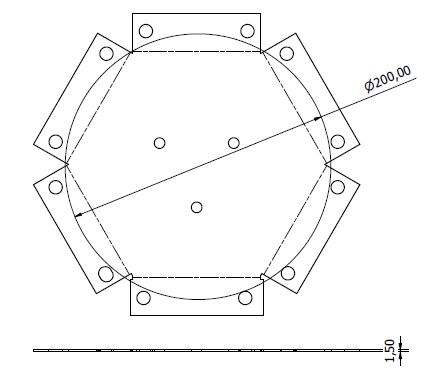
\includegraphics[width=0.6\linewidth]{Figures/Flat}
	\caption[Moving Platform]{Moving Platform (Flat Pattern)}
	\end{figure}
\end{center}

The moving platform has flanges to provide linking points of the Stewart Platform legs. A flange of 30mm is considered allows ample space for the spherical joint (whose connecting side diameter is 10mm) to fit and to be well centred.
\begin{center}
	\begin{figure}[H]
	\centering
	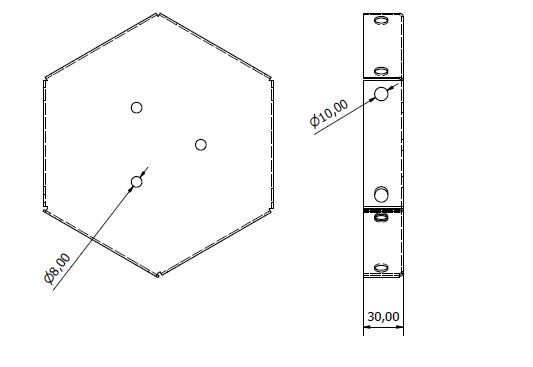
\includegraphics[width=0.6\linewidth]{Figures/Folded}
	\caption[Moving Platform]{Moving Platform (Folded)}
	\end{figure}
\end{center}

Both stainless steel and mild steel would make a suitable base for the Stewart platform due to their weight. They are also easy to machine (machinability for Mild steel - 78 per cent, for stainless steel: 45 - 110 per cent). Mild steel is readily available in the Kenyan market. Stainless steel is a bit more expensive.

Due to cost constraints and for the Stewart platform's overall weight (and without compromising on the platform stability), aluminium can be used to manufacture the base. A thickness of 2.5mm for the base is used.
\begin{center}
	\begin{figure}[H]
	\centering
	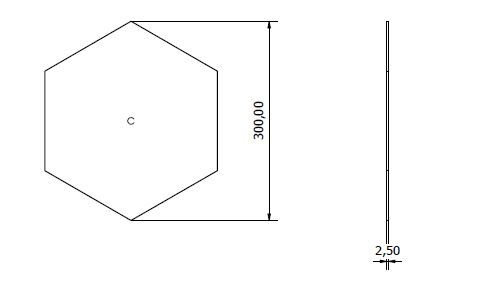
\includegraphics[width=0.6\linewidth]{Figures/Base}
	\caption[Base Plates]{Base Plates}
	\end{figure}
\end{center}
Aluminium, unlike mild steel, would not require post-processing methods (e.g. powder coating) which would add on the cost.
\subsubsection{Sensing Bars/Rods}
Two options can be considered:
\begin{itemize}
\item Bars with square cross-section
\item Cylindrical bars
\end{itemize}
Cylindrical bars are preferable due to their ease of coupling with the available spherical joints. Cylindrical bars also guarantee uniform deformation of the bars - both in the axial and cross-sectional directions.

From inquiries around suppliers in the Kenyan Market, these bars are usually available in steel and aluminium. In order to select the optimum solution for this application, the Yield Strength, modulus of rigidity, Young's Modulus and density of both materials are compared. The different values are shown in table \ref{tabmat}. 
\begin{table}[!h]
\caption[Aluminium and Steel Properties]{Material Properties of Aluminium and Steel}
\label{tabmat}

\begin{tabular}{|l|l|l|l|l|}
\hline
\textbf{Material} & \textbf{Yield Strength (MPa)} & \textbf{G (GPa)} & \textbf{E (GPa)} & \textbf{Density ($g/cm^3$)}\\
\hline
Steel & 240 & 79 & 190 - 215 & 7.8\\
\hline
Aluminium & 270 & 26 & 69 - 70 & 2.7\\
\hline
\end{tabular}
\end{table}

E - Young's Modulus\\
G - Modulus of Rigidity

From $ \sigma = E \epsilon $, where $\sigma$ - Stress , E - Young's Modulus and $ \epsilon$ - Strain, materials with high values of Young Modulus will give smaller values of strain when subjected to a deforming force. Thus, aluminium rods will experience higher strains than steel rods.

Materials with high modulus of rigidity will require huge amounts of force to deform. Aluminium rods will experience deformation under small amounts of force as compared to steel rods.

Aluminium rods have the capability of bearing higher loads before their deformation goes from elastic to plastic as compared to steel rods. Aluminium rods also have the benefit of being lightweight.

%\section{Sensing Rods Design - Length}
%From the previously selected dimensions i.e diameter of platform, diameter of base and distance between the base and platform, the length of each rod can be determined by geometry.

%Rod length = 140mm
%\begin{center}
%	\begin{figure}[!h]
%	\centering
%	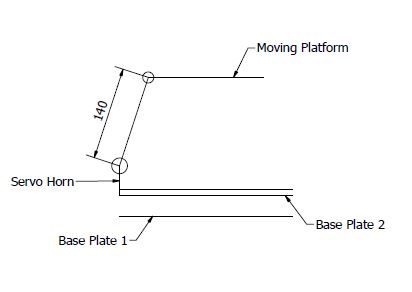
\includegraphics[width=0.6\linewidth]{Figures/Ideation}
%	\caption[Ideation]{Ideation technique to obtain rod length}
%	\end{figure}
%\end{center}

\subsubsection{Sensing Rods Design - Shape}
Two options can be considered:
\begin{itemize}
\item Solid cylindrical rods
\item Hollow Cylindrical rods
\end{itemize}
From local suppliers, 10mm aluminium rods are available and economical. The rods are not hollow. From $\sigma = \frac{F}{A}$, where $\sigma$ - Stress, F - Axial Force on the leg and, A - Cross-sectional area, for the same amount of axial load, the hollow rod will experience more stress and consequently larger strains as compared to the solid rod. The rods are threaded at the ends for coupling with the spherical joints.

If solid rods are used, strain gauges of high sensitivity should be used.
\begin{center}
	\begin{figure}[H]
	\centering
	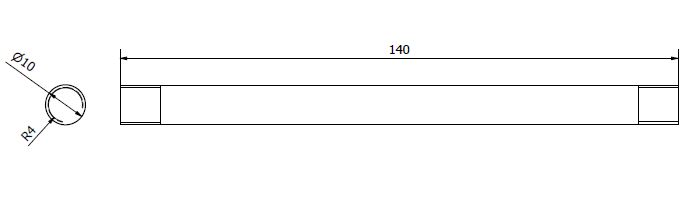
\includegraphics[width=0.8\linewidth]{Figures/Rod}
	\caption[Aluminium rod]{Aluminium rod}
	\end{figure}
\end{center}

\subsubsection{Test Flange and Strut}
The test flange will be used to hold the strut during wind tunnel testing. For optimum results, the reference axis is taken to be in the middle of the middle platform \cite {fernandes_design_nodate}. The flange will be fastened to the moving platform by use of bolts and nuts. Fasteners are more economical and easy to achieve as compared to welding. M6 or M8 nuts can be used for this purpose.

The test flange should hold the strut for a considerable length in order to keep the rotation of the strut below certain predefined values and thus limiting torsion and bending behaviour of the strut during Wind Tunnel testing.
\begin{center}
	\begin{figure}[H]
	\centering
	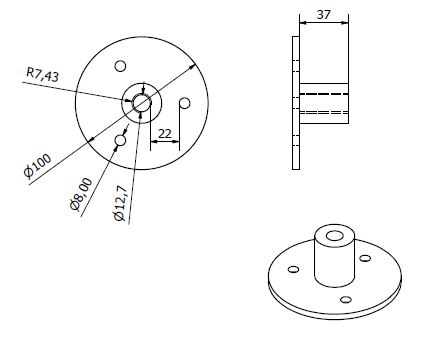
\includegraphics[width=0.75\linewidth]{Figures/Test}
	\caption[Test flange]{Test flange design}
	\end{figure}
\end{center}
The strut will go into the test section of the Wind tunnel at the Fluids lab in JKUAT. The strut should be long enough to position the model under testing in the middle of the test section. The strut will also be subjected to the flow forces in the wind tunnel. It should therefore be made of as small diameter as possible. The strut dimensions of diameter 12.5mm and a length 400mm are practical, based on the Wind Tunnel set-up (Appendix).
\begin{center}
	\begin{figure}[H]
	\centering
	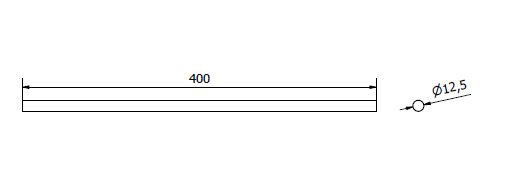
\includegraphics[width=0.75\linewidth]{Figures/Strut}
	\caption[Strut]{Strut}
	\end{figure}
\end{center}

\subsubsection{Spherical Joints}
For the 6-6 type, both platforms have six vertices and
the connections between the sensing bars and the platforms is made by simple spherical joints. Single spherical joints are preferable because they are easy to manufacture and they eliminate the issues of interference between sensing bars when double spherical joints are used \cite{fernandes_design_nodate}.  

Connection with spherical joints also prevents the torsion and bending phenomena in the bars when subjected to axial forces \cite{fernandes_design_nodate}.

Spherical joints can be obtained from online stores. One such store is RS Components Africa. Options of spherical joints to choose from include:
\begin{itemize}
\item Ball and socket joint M5
\item Ball and socket joint M6
\item Ball and socket joint M8
\item Ball and socket joint M10
\end{itemize}
Based on the diameter of the available aluminium rods, Ball and socket joint M10 is used.
\begin{center}
	\begin{figure}[H]
	\centering
	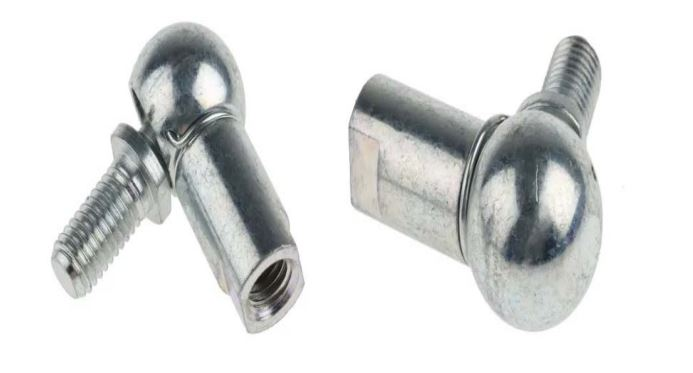
\includegraphics[width=0.6\linewidth]{Figures/Spherical}
	\caption[Spherical Joint]{Spherical Joint available from RS Components Africa \cite{datasheet_spherical}}
	\end{figure}
\end{center}
The following dimensions are provided by the manufacturer:
\begin{center}
	\begin{figure}[H]
	\centering
	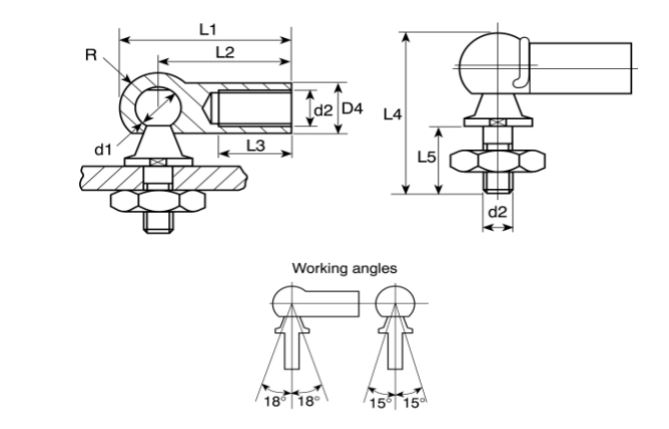
\includegraphics[width=0.8\linewidth]{Figures/Spherical Dimensions}
	\caption[Spherical Joint Dimensions]{Spherical Joint Dimensions \cite{datasheet_spherical}}
	\end{figure}
\end{center}
\begin{table}[H]
\caption{Spherical Joint Dimensions}
\end{table}
\begin{tabular}{|l|l|l|l|l|l|l|l|l|l|l|l|}
\hline
\textbf{Size(mm)}& \textbf{D1}& \textbf{D2}&\textbf{ D4}& \textbf{L1}& \textbf{L2}& \textbf{L3}& \textbf{L4}& \textbf{L5}& \textbf{R} & \textbf{A/F} & \textbf{min pull-off Force(N)}\\
\hline
10 & 16 & M10 & 16 & 47 & 35 & 15.5 & 47.5& 20 & 12 & 13 & 80\\
\hline
\end{tabular}

\paragraph{}

The Spherical joint was done on Autodesk Inventor and included in the Stewart Platform Assembly.
\begin{center}
	\begin{figure}[H]
	\centering
	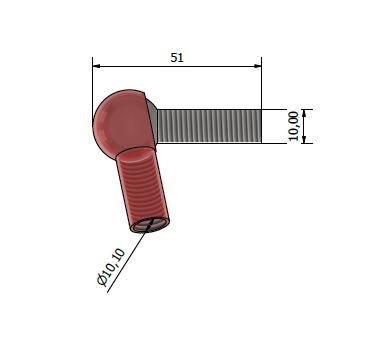
\includegraphics[width=0.5\linewidth]{Figures/Spherical CAD}
	\caption[Spherical Joint CAD]{Spherical Joint as designed on Autodesk Inventor}
	\end{figure}
\end{center}
\subsubsection{Finite Element Analysis}
A Finite Element Analysis was done on the Stewart platform design to determine its performance under given loads. The platform is going to be subjected to a force during wind tunnel testing. A maximum load of 50N is selected for the Finite Element Analysis. This could be more or less since models vary in size. The z-component of the force is considered. 
The mesh generated is shown in the figure \ref{fig:feamesh}.
\begin{center}
	\begin{figure}[H]
	\centering
	\includegraphics[width=0.75\linewidth]{Figures/FEA}
	\caption[Stewart platform mesh]{Stewart platform mesh}
	\label{fig:feamesh}
	\end{figure}
\end{center}
The rods/legs of the Stewart platform are subjected to axial forces which cause slight strains which can be used to obtain force and moment measurements during wind tunnel testing.
\clearpage
\begin{center}
\begin{table}[H]
\caption{Operating Conditions}
\centering
\end{table}
\begin{tabular}{|l|l|}
\hline
\textbf{Load Type} & \textbf{Force}\\
\hline
Magnitude & 50.0N\\
\hline
Vector X & 7.794N\\
\hline
Vector Y & -48.206N\\
\hline
Vector Z & 10.745N\\
\hline
\end{tabular}
\end{center}

\begin{center}
\begin{table}[!h]
\caption[FEA Setup]{Other FEA setup parameters}
\centering
\end{table}
\begin{tabular}{|l|l|}
\hline
Constraint & Fixed\\
\hline
Materials & Aluminium 6061\\
 & Stainless steel\\
\hline
Contacts & All bonded\\
\hline
Mesh& Avg element size: 0.1mm\\
& Minimum element size: 0.2mm\\
& Grading Factor: 1.50\\
& Maximum turn angle: 60 deg\\
\hline
\end{tabular}
\end{center}
\subsubsection{Inverse Kinematics of a Stewart Platform}
This is the calculation of each leg length based on the desired position of the Stewart platform. 
For the Stewart platform, the translation $^{p}T_{b}$ from the base origin to the platform origin can be described with a single vector T = $(t_{x} t_{y} t_{z})^{T} $. The rotation of the platform can be denoted as $^{p}R_{b}$. Thus the following relationship for the frame of reference can be stated \cite{Eisele_2019}:
$$^{p}T_{b} = T$$
	$$^{p}R_{b} = R$$
	$$^{b}T_{p} =(^{p}T_{b})^{-1} =T^{-1}$$
	$$^{b}R_{p} = (^{p}R_{b})^{-1} $$
\begin{center}
	\begin{figure}[!h]
	\centering
	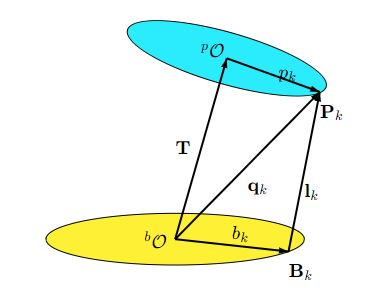
\includegraphics[width=0.4\linewidth]{Figures/servo2}
	\caption[Leg length]{Leg Length \cite{Eisele_2019}}
	\end{figure}
\end{center}
The leg length $l_{k}$ can therefore be found with:
\begin{ceqn}
\begin{align}
	l_{k} = P_{k} - B_{k} = T + R \times p \times R^{-1} - b_{k}
\end{align}
\end{ceqn}
Where,\\
$P_{k}$ - leg attachment on platform \\
$B_{k}$- leg attachment on base 
\subsubsection{Inverse Kinematics Using Rotational Servo Motors}
For a rod of fixed length d between servo horn anchor $H_{k}$ and platform anchor $P_{k}$.  $H_{k}$ has a distance h between the original base anchor and servo shaft $B_{k}$. The vector h is perpendicular to the servo shaft and is rotated by angle $\alpha_{k}$ when lifted from the horizontal line.
\begin{center}
	\begin{figure}[!h]
	\centering
	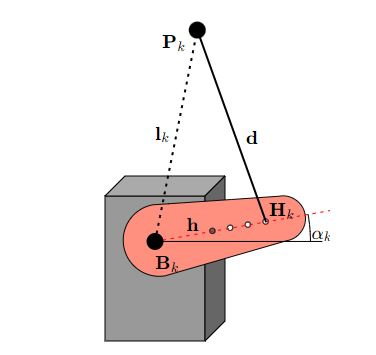
\includegraphics[width=0.4\linewidth]{Figures/servo}
	\caption[Servo angle]{Servo angle \cite{Eisele_2019}}
	\end{figure}
\end{center}
Further, looking from the top onto the base, each servo can be rotated by the angle $\beta_{k}$ in addition to its position $B_{k}$. The servo shaft $s_{k}$ moves in the x-y plane and is orthogonal to the vector h.
\begin{center}
	\begin{figure}[!h]
	\centering
	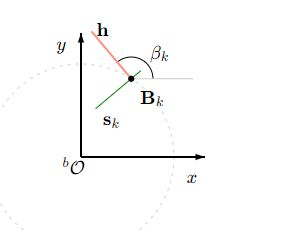
\includegraphics[width=0.4\linewidth]{Figures/servo1}
	\caption[Planar view]{Planar view \cite{Eisele_2019}}
	\end{figure}
\end{center}
The anchor $H_{k}$ can be calculated as we rotate around the z-axis with angle $\beta_{k}$ and  by $-\alpha_{k}$ around the y-axis to lift the servo horn which lies in the local x-axis \cite{Eisele_2019}.
\begin{ceqn}
\begin{align}
	H_{k} = B_{k} + R_{z}(\beta_{k}) R_{y}(-\alpha_{k})\begin{pmatrix}
	|h|\\ 0 \\ 0
	\end{pmatrix}
	\label{eq:myeqn2}
\end{align}
\end{ceqn}
\begin{ceqn}
 \begin{align}
	= B_{k} + |h|\begin{pmatrix}
	cos(\alpha_{k})cos(\beta_{k})\\
	 cos(\alpha_{k})sin(\beta_{k})\\
	  sin(\alpha_{k})
	\end{pmatrix}
	\label{eq:myeqn2}
\end{align}
\end{ceqn}
Carrying out the same procedure but with the servo arm when it is on the opposite side and we have:
\begin{ceqn}
\begin{align}
	H_{k} = B_{k} + R_{z}(\beta_{k}) R_{y}(\pi -\alpha_{k})\begin{pmatrix}
	-|h|\\ 0 \\ 0
	\end{pmatrix}
	\label{eq:myeqn2}
\end{align}
\end{ceqn}
\begin{ceqn}
	\begin{align}
	= B_{k} + |h|\begin{pmatrix}
	cos(\alpha_{k})cos(\beta_{k})\\
	 cos(\alpha_{k})sin(\beta_{k})\\
	  sin(\alpha_{k})
	\end{pmatrix}
	\label{eq:myeqn2}
\end{align}
\end{ceqn}
Squaring the lengths of h, d, $l_{k}$ we get the relationship:
\begin{ceqn}
	\begin{align}
		h^2 = (H_{k}-B_{k})^{T}(H_{k}-B_{k})
	\end{align}
\end{ceqn}
\begin{ceqn}
	\begin{align}
		d^2 = (P_{k}-H_{k})^{T}(P_{k}-H_{k})
	\end{align}
\end{ceqn}
\begin{ceqn}
	\begin{align}
		l_{k}^2 = (P_{k}-B_{k})^{T}(P_{k}-B_{k})
	\end{align}
\end{ceqn}
From the above relationships, further derivation and trigonometric substitutions are done to obtain the inverse kinematics used to calculate each servo angle. This is given as \cite{Eisele_2019}:
\begin{ceqn}
\begin{align}
	\alpha_{k} = sin^{-1}(\frac{g_{k}}{\sqrt{e_{k}^2+f_{k}^2}})-arctan2(f_{k}, e_{k})
\end{align}
\end{ceqn}
Where,
$$e_{k} = 2hl_{k}^{(z)} $$
$$e_{k} = 2h(cos(\beta_{k})I_{k}^{(x)}+sin({\beta_{k}})I_{k}^(y))$$
$$g_{k} = l_{k}^2 - (d^2 - h^2)   $$

\subsection{Electromechanical Design}
Two methods of actuation are popular with Stewart platforms:
\begin{itemize}
\item Linear actuators
\item Use of motors
\end{itemize}
Whereas linear actuators are relatively easy to control, they are very expensive. Thus the choice of motors.
%\subsection{Servo Horn}
%This will provide the connection between the motor and the spherical joints hence the aluminium rods. An 8mm hole on one end for mounting the spherical joint and another hole 8.5mm that will allow coupling with the servo arm bush of 8.6mm. The 1mm gap ensure tight fitting.
%\begin{center}
%	\begin{figure}[!h]
%	\centering
%	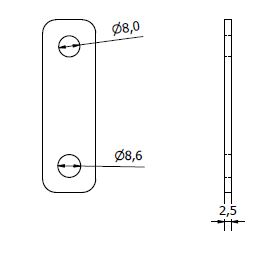
\includegraphics[width=0.6\linewidth]{Figures/Horn}
%	\caption{Servo horn}
%	\end{figure}
%\end{center}

\subsubsection{Motor Selection}
One parameter was considered in our motor selection i.e. torque required. From the Autodesk Inventor design environment, the mass of the moving platform and mechanical couplings was 2.6kg. Each motor is supposed to move a minimum mass of 0.177kg. Using a servo horn of distance 45mm centre-to-centre, and Distance = $ \pi $ D, then:
\begin{ceqn}
\begin{align}
	Torque = (0.1777 \times 9.81)\times \frac{141.37}{1000} = 0.246 N\cdot m
\end{align}
\end{ceqn}
Motors of minimum torque of 0.2 N $\cdot m$ were considered. But for control considerations, only stepper motors and servo motors were shortlisted. Servo motor was considered over Stepper motor because they are cheaper. Also, we are only interested in 0 - 180 degrees positions.

The Servo motor \textbf{TowerPro SG5010} is suitable for this project. The specifications provided by the manufacturer are as follows:

\begin{table}[!h]
\caption[Motor Specifications]{TowerPro SG5010 Specifications}
\end{table}
\begin{center}
\begin{tabular}{|l|l|}
\hline
\textbf{Model}& TowerPro SG5010\\
\hline
\textbf{Operating Voltage} & 4.8V - 6.6V\\
\hline
\textbf{Operating Speed @ 4.8V} & 0.20sec/60$^{\circ}$\\
\hline
\textbf{Operating Speed @ 6.6V}& 0.16sec/60$^{\circ}$\\
\hline
\textbf{Stall torque @ 4.8V} & 5.5 kg-cm or 0.54 N $\cdot$ m\\
\hline
\textbf{Stall torque @ 6.6V} & 6.5 kg-cm or 0.64 N $\cdot$ m\\
\hline
\end{tabular}
\end{center}
Prices range between \textbf{Ksh.700} and \textbf{Ksh.1400}

\subsubsection{Design of the Force Sensor}
The force sensor module will be used to measure the force and moments from the aerodynamic loads applied on model being tested in the wind tunnel. The forces to be measured are the drag, lift and thrust as well as associated moments. For this subsystem two possible conceptual designs are to be considered:
\begin{itemize}
\item External force sensor
\item Stewart Platform as a force sensor
\end{itemize}
\subsubsection*{External Force Sensor}
In this case it would require at least 3 orthogonally positioned load cells measuring each force component. Each load cell would be mechanically linked to the model such that forces experienced on each axis are measured by each load cell as shown in figure \ref{fig:balex}. 
\begin{center}
	\begin{figure}[H]
		\centering
		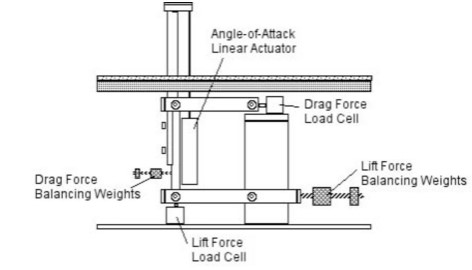
\includegraphics{Figures/modBal}
		\caption[Diagram of a force balance]{Diagram of a force balance \cite{post_force_2010}}
		\label{fig:balex}
	\end{figure}
\end{center}
This configuration is, however, bulky since it requires an additional external system for force measurements in addition to the Stewart platform for positioning the model. This is however complemented by the simplicity in calibration of the load cells and does not require a complex force transformation matrix and other issues with force amplification created by the use of an integrated system.
\subsubsection*{Stewart Platform as a force sensor}
In this configuration the Stewart platform legs are used as force sensors by attaching strain gauges on the legs of platform. Similar work has been done by \cite{ferreira2015design} without the use of actuators as is proposed in this project. Using the Stewart platform as a force sensor requires the actuators to be locked with zero degrees of freedom.

Four strain gauges are required for each leg for a full Wheatstone bridge configuration. 
\begin{center}
	\begin{figure}[H]
		\centering
		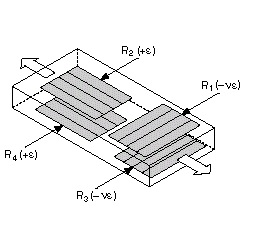
\includegraphics{Figures/loadConf}
		\caption[Strain Gauge Configuration]{Strain Gauge Configuration \cite{noauthor_measuring_nodate}}
		\label{strain}
	\end{figure}
\end{center}
In this case, as shown in figure \ref{strain}, the load cells are able to measure the axial strain on each leg. R1 and R3 are active strain gauges measuring the compressive Poisson effect (–νe). R2 and R4 are active strain gages measuring the tensile strain (+e). The output generated from the Wheatstone bridge is then amplified and read to determine the strain on each leg.
In the case of this project, a full bridge strain gauge sensor with each strain gauge orthogonally positioned allowing for elimination of noise and measurement of the strain axially on each rod is used.

%\paragraph{Force measurement Circuit}
\subsubsection*{Force measurement Circuit}

The output excitation of the Wheatstone bridge needs to be amplified as it results in low outputs. An analogue to digital converter is also required for the analogue to digital converter. Some considerable options are the HX711 or the AD7193 converters which may be used as digital to analogue converters. The AD7193 is designed for high precision and has a delta sigma filter to remove noise from measurements.  However, the AD7193 was not used due to it's high cost compared to the HX711 regardless of the advantage it offers with serial peripheral Interface communication allowing for multiple modules on the same bus.

The connection of the AD7193 to the microcontroller will be via Serial Peripheral Interface (SPI). The configuration is as shown in figure \ref{spi}:
\begin{center}
\begin{figure}[H]
\centering
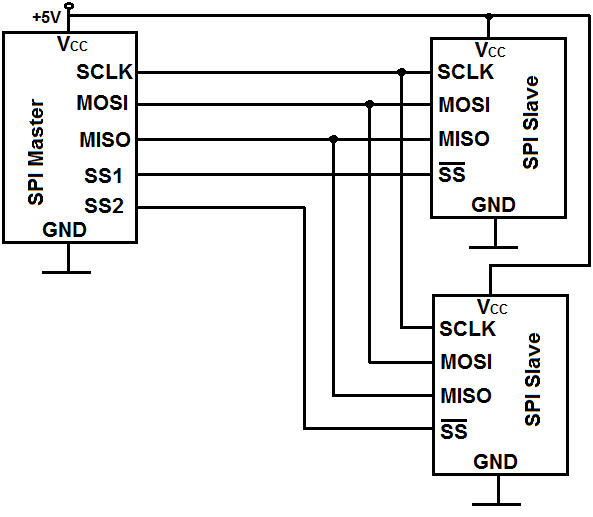
\includegraphics[width=0.55\linewidth]{Figures/SPI}
\caption[SPI configuration]{SPI configuration}
\label{spi}
\end{figure}
\end{center}
In this configuration the when the chip select pin of an amplifier is set to low, the microcontroller is able to obtain data from that strain gauge. This configuration allows for a four wire interface to connect to six strain gauge sensors and obtain measurements.

The HX711 however allows for the I2C like communication via two wires (serial clock (SCL) and Serial Data (SDA)). They however do not have hardware addresses thus many pins are required for the interface, This can however be remedied by the use of a shared SCL between each of the amplifier modules reducing the overall number of pins required to interface.

\subsubsection*{Force transformation matrix} 
In such a case the forces experienced at the top of the platform are distributed between the 6 legs and as result, a force transformation matrix is required to resolve the forces applied on each axis as measured by each load cell on each leg. 

The forces experienced by the legs can be expressed as:
\begin{ceqn}
\begin{align}
	\begin{Bmatrix}
		\vec{F}_e \\
		\vec{M}_e \\
	\end{Bmatrix} = [H]\{F\}
\end{align}
\end{ceqn}

Where 
\begin{itemize}
\item $\vec{F}_e $ - external force applied to the platform
\item $\vec{M}_e$ - external moment applied to the platform
\item H - transformation matrix which relates measured forces and applied forces
\item F - axial force
\end{itemize}  
The derivation has been done and is presented in the appendix.


\subsection{Velocity Measurement}
An important part in wind tunnel measurements is the measure of pressure at specific points in the wind tunnel and computing the corresponding air speed. This is achieved by the use of a pitot probe. 
\begin{center}
\begin{figure}[H]
\centering
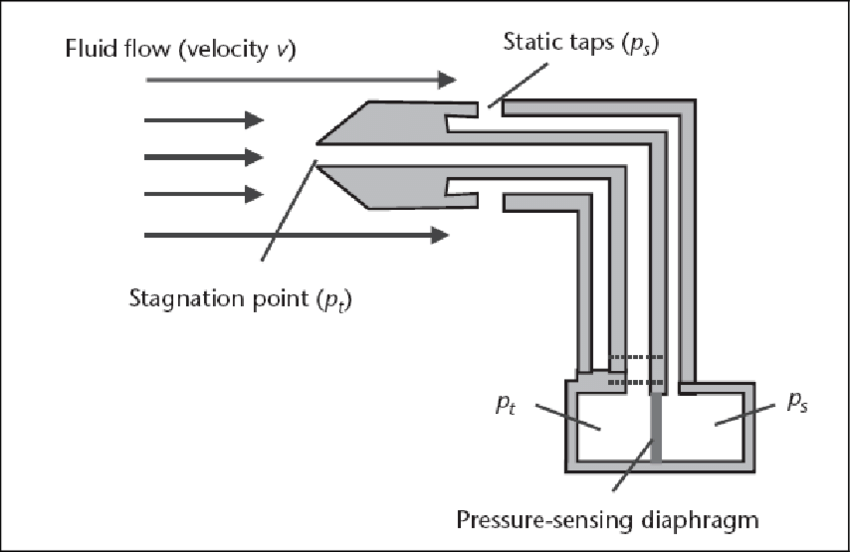
\includegraphics[width=0.6\linewidth]{Figures/pitot}
\caption[Pitot-static tube]{Pitot-static tube \cite{viquerat_continuous_2006}}
\end{figure}
\end{center}
For steady flow of an incompressible fluid for which viscosity can be neglected, the fundamental equation has the form\cite{viquerat_continuous_2006}:

\begin{ceqn}
	\begin{align}
	v = \sqrt{\frac{2(P_{0} - P)}{\rho}}
\end{align}
\end{ceqn}

Where V is the speed of the fluid, $P_{0}$ is the total, also called the stagnation, pressure at that point of measurement, and P is the static pressure at the same point.

Three pitot probes are to be used in the wind tunnel i.e. in the test section, intake and diffuser sections.
                                                                                                                                                                   
\begin{center}
\begin{figure}[H]
\centering
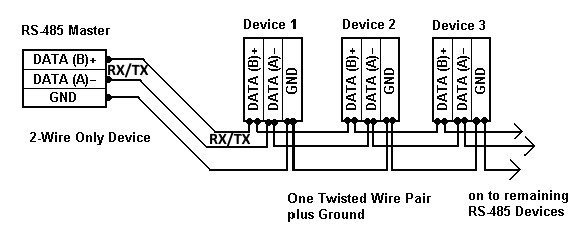
\includegraphics{Figures/modbus}
\caption[RS485 communication]{RS485 communication}
\label{fig:rs485}
\end{figure}
\end{center}
Module communicates to the microcontroller using a TTL to RS485. Each module is individually addressable further simplifying the interface as shown in figure \ref{fig:rs485}. 
The protocol allows for long distance serial communication and interface with multiple devices on the same bus.

\subsection{Control system}
This section deals with the control of the stewart platform. It involves allowing input and obtaining output form the platform force balance.
\subsubsection{Human Machine Interface}
The purpose of the interface is to enable control of the platform position as well as to obtain measured data from the strain gauges and pitot tubes. 
The general layout is as shown in the figure \ref{fig:hmi}:
\begin{center}
\begin{figure}[H]
\centering
\includegraphics{Figures/Interface}
\caption[Human Machine Interface]{Human Machine Interface}
\label{fig:hmi}
\end{figure}
\end{center}

The primary interface between the microcontroller is wireless. 
For this interface two transport methods were considered: User Datagram Protocol (UDP) and Transmission Control protocol (TCP).
UDP is a communications protocol that is primarily used to establish low-latency and loss-tolerating connections.
 TCP on the hand does not experience data loss and in our case the use of protocol buffers as a means of serialization of messages to binary saving on bandwidth. 
 TCP requires only one initial handshake between the server and client, after which messages can be transmitted continuously (streaming).
 Due to assurance of data integrity (no loss) and lower bandwidth use thus higher data transfer rates, TCP was chosen as the main protocol.
  This allows for high speed low latency communication without need for a wired connection. It also allows for bidirectional streaming of information thus allowing for both control input and output of measured values. The interface is to enable the abstraction of data acquisition and actuator control to a simple interaction with buttons and other visual interfaces available in a computer program.

The decoupling of the microcontroller and the program to be hosted on the desktop allows for advanced data processing such as application of filters and resolving measurements into usable information. It also allows for the use of more powerful processor and high level programming languages to more effectively perform complex calculations without taking a toll the sensor sampling rate that would occur with on board processing in the microcontroller.

A user interface was also required to record user input and display incoming data.
\subsubsection{Control Algorithm}
\begin{center}
	\begin{figure}[H]
	\centering
	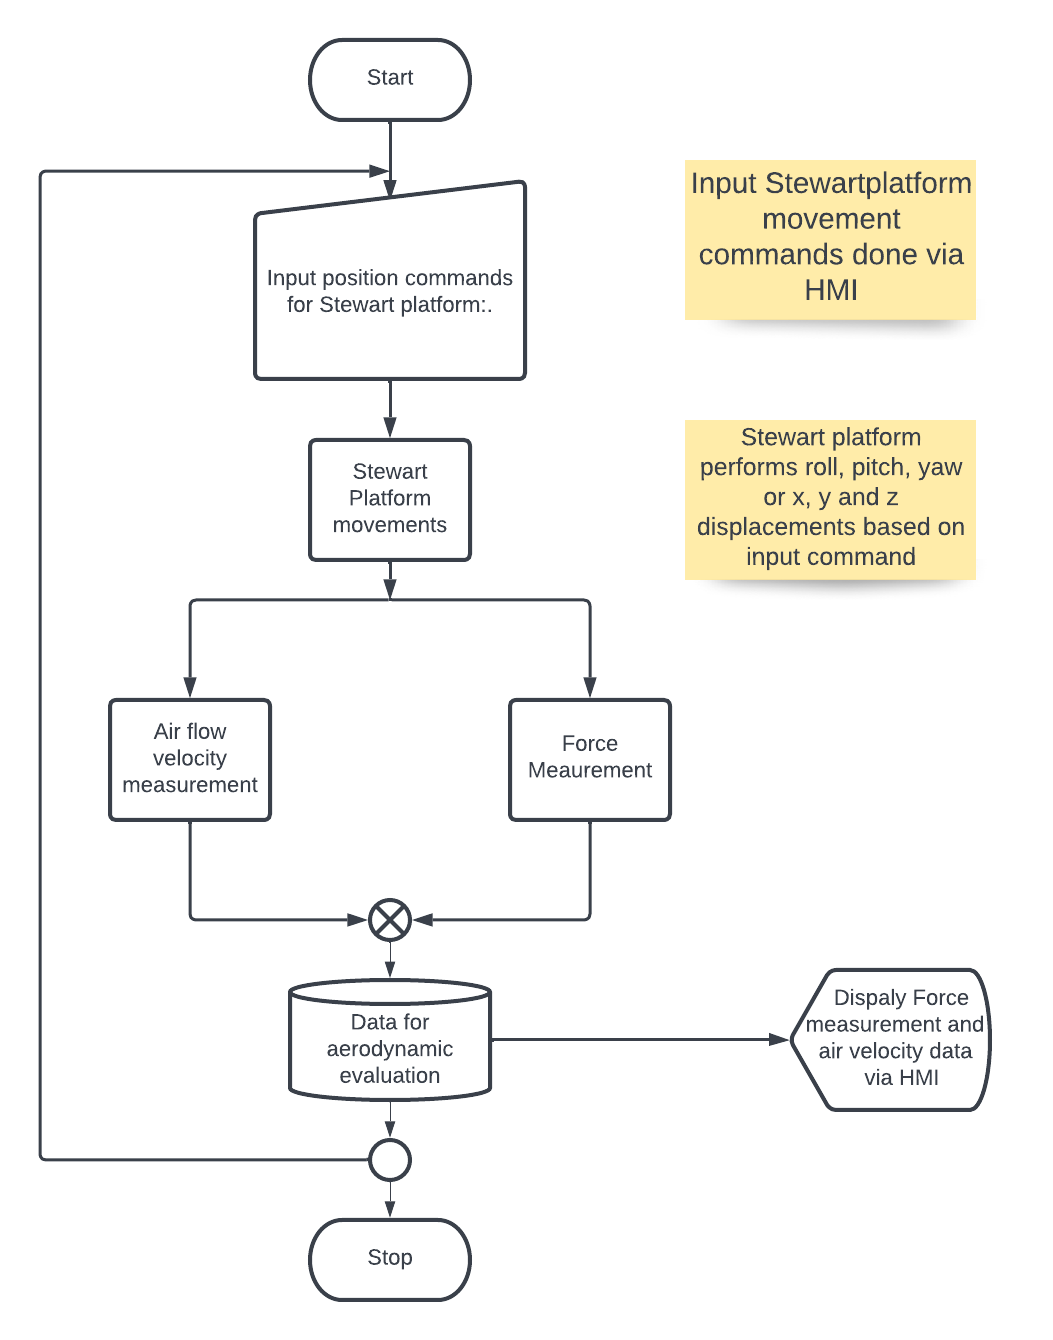
\includegraphics[width=0.7\linewidth]{Figures/Flow}
	\caption[Control Algorithm]{Control Algorithm for the Stewart Platform with Force Measurement}
	\end{figure}
\end{center}
\subsection{Electrical Design}
This section looks at the required electrical connections to make the system functional and interface with the control unit.
\subsubsection{Printed Circuit Board Design}
This section looks at the design of the circuits used to power and get readings from the sensors and control the actuators.

\subsubsection{Microcontroller}
The main requirement for this is the need for wireless communication via WIFI and large number of I/O interface at cost effective rate. This brings down the options to the ESP32 and Raspberry Pi RP2040. Both are dual core devices which are feature rich however the raspberry rp2040 only has 28 I/O pins while the ESP32 has 34 pins and due to this the ESP32 was chosen. 
\begin{center}
	\begin{figure}[H]
	\centering
	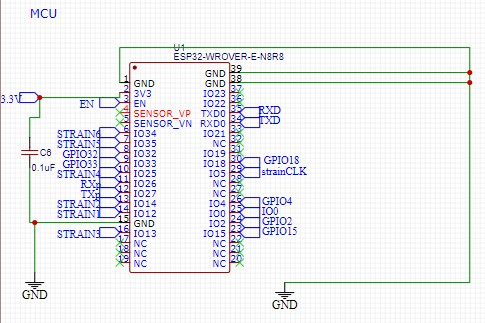
\includegraphics[width=0.7\linewidth]{Figures/mcu}
	\caption[Microcontroller]{Microcontroller}
	\end{figure}
\end{center}
\subsubsection{Power Supply}
The power supply chosen is an AC/DC power converter since the highest voltage required is 12 volts. This is also used as the highest power supply to the PCB.

Both 5 and 3.3 volts are required in the PCB for other peripherals. To this end, a buck converter and linear converter are used for 5 ad 3.3 volts respectively.

\begin{center}
	\begin{figure}[H]
	\centering
	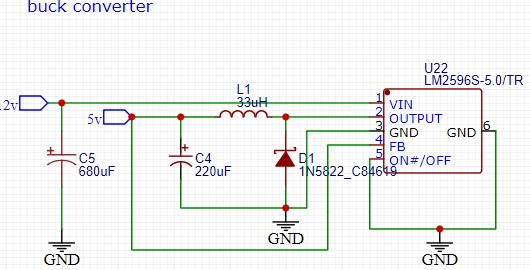
\includegraphics{Figures/buck}
	\caption[Buck converter]{Buck Converter 12V to 5V}
	\end{figure}
\end{center}

\begin{center}
	\begin{figure}[H]
	\centering
	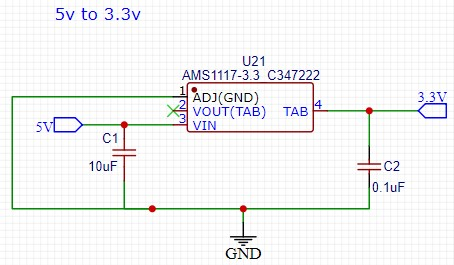
\includegraphics{Figures/5233}
	\caption[Linear Voltage Converter]{Linear level converter 5V to 3.3v}
	\end{figure}
\end{center}
The linear converter dissipates the energy loss though heat while buck converter is through switching.

\subsubsection{Servo Control}
Since the microcontroller used (ESP32) is based on 3.3V logic. There is a need for 5V logic to control the servos and thus a bidirectional logic level converter is utilized which leverages an internal drain N-channel MOSFET. 
\begin{center}
	\begin{figure}[H]
	\centering
	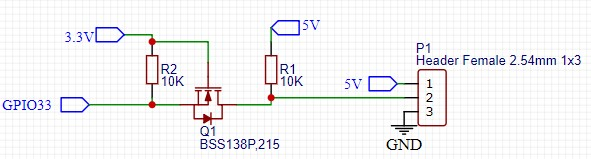
\includegraphics{Figures/logik}
	\caption[Bidirectional Logic Level converter]{Bidirectional Logic Level converter}
	\label{fig:logik}
	\end{figure}
\end{center}
The configuration designed is shown in figure \ref{fig:logik}